\chapter{从论文配图到汇报与海报}

材料学博士生小周在第 9 章完成了钙钛矿太阳能电池界面改性论文的 Figure 2。那是一张双栏通栏的四面板组图：面板 a 交代平面器件的七层结构与钝化层位置，面板 b 给出截面层序的模型生成示意，面板 c 对比对照与改性器件的电流密度—电压（$J\text{--}V$）曲线，面板 d 展示连续光照 $1000\ \text{h}$ 内的归一化功率转换效率（PCE）衰减。整张图在 $174\ \text{mm}$ 印刷宽度下字号统一为 $8\ \text{pt}$，色彩与线型相互呼应，发给合作者审阅时获得了好评。

两周后，小周要在课题组大组会上作 10 分钟进展汇报；一个月后，他还要带一张 A0 竖版海报参加学术年会。为了省事，他把论文里的 Figure 2 整张截图拖进 16:9 幻灯片，在页面顶部打上“结果”两个大字（后文图~\ref{fig:ch12-05}a 将按后排视角还原这一页的效果）。到了组会现场，坐在会议室最后一排的同门眯着眼睛也看不清横纵坐标的数字；小周刚讲完面板 a 的器件层序准备切入效率对比，导师却打断他问：“右边那张图里哪条线是对照？面板 b 那张电镜图是你自己拍的吗？”原来，论文图注没有跟着截图进幻灯片，而面板内的标注在缩放与重采样后变得模糊不清。

组会结束后，小周又开始排会议海报。他把论文的摘要、引言、方法和结论按三栏原样贴满画布，再把那张四面板组图等比放大塞进海报正中央。把草稿缩略图发给师姐看时，师姐只问了一句：“如果有人从展板通道走过去，五秒钟内能看出你到底改了哪一层、效率提高了多少吗？”

小周手里的科学证据没有任何变化，为什么在论文里合格的组图，到了报告厅和海报展区却接连失效？原因在于论文、口头汇报和学术海报面对的是三种截然不同的观看条件。本章围绕同一项钙钛矿界面改性研究（采用标准单二极管模型生成的模拟教学数据），系统讲解如何用视角换算确定字号与线宽，如何把四面板论文组图拆解为逐步揭示的 16:9 汇报页，如何按三层阅读距离规划 A0 竖版海报，以及如何在 \scidraw{} 中完成重绘、模板排版与跨版本一致性核验。

\section{同一研究，三种观看条件}

很多研究者在准备学术报告或会议海报时，习惯把它们当成“论文的缩减版”——从论文文档里挑几张图、复制几段话，塞进不同尺寸的画布里。这种做法忽略了一个基本事实：读者在书桌前读论文、听众在报告厅看投影屏幕、参会者在展厅通道里浏览海报，这三种场景在\textbf{观看距离、可用时间、节奏由谁控制}三个物理与认知变量上存在数量级的差异（图~\ref{fig:ch12-01}）。

\begin{figure}[htbp]\centering
\resizebox{\linewidth}{!}{% FIG ch12-01 three viewing conditions (Chinese)
\begin{tikzpicture}[
  x=1mm, y=1mm,
  font=\sffamily\small,
  text=BookInk,
  coltitle/.style={font=\sffamily\bfseries, text=BookTeal, align=center},
  cell/.style={draw=BookRule, fill=white, align=left, text width=42mm, inner sep=2mm, minimum height=9mm},
  emphcell/.style={cell, fill=BookPale, draw=BookTeal, font=\sffamily\bfseries\small},
  icon/.style={draw=BookInk!40, fill=BookPale, line width=0.5pt},
]
  % Column headers with scale icons (1 m bar shared)
  \def\colX{22, 72, 122}
  \foreach \x/\name/\w/\h in {22/论文/42/59, 72/汇报/64/36, 122/海报/42/59} {
    \begin{scope}[shift={(\x, 108)}]
      \node[coltitle] at (21, 14) {\name};
      \draw[icon, fill=white] (6, 0) rectangle ++(\w, \h);
      \ifnum\x=72
        \draw[BookInk!60, line width=0.8pt] (10, 4) -- (54, 4);
        \draw[BookInk!60, line width=0.8pt] (10, 32) -- (54, 32);
      \fi
    \end{scope}
  }
  \draw[BookTeal, line width=1pt] (10, 100) -- ++(20, 0);
  \node[font=\scriptsize, anchor=west] at (32, 100) {1 m（比例尺）};

  \node[cell, anchor=north west] at (0, 98) {观看距离};
  \node[cell] at (22, 89) {30--50 cm};
  \node[cell] at (72, 89) {2--15 m};
  \node[cell] at (122, 89) {先 2--5 m\\再 0.5--1.5 m};

  \node[cell, anchor=north west] at (0, 78) {可用时间};
  \node[cell] at (22, 69) {读者自定};
  \node[cell] at (72, 69) {每页约 1--2 分钟};
  \node[cell] at (122, 69) {几秒决定是否停留\\停留后数分钟};

  \node[cell, anchor=north west] at (0, 58) {节奏控制};
  \node[cell] at (22, 49) {读者};
  \node[cell] at (72, 49) {讲者};
  \node[cell] at (122, 49) {观众};

  \node[cell, anchor=north west] at (0, 38) {谁来解释};
  \node[cell] at (22, 29) {图注};
  \node[cell] at (72, 29) {讲者};
  \node[cell] at (122, 29) {海报自身};

  \node[emphcell, anchor=north west] at (0, 18) {内容策略};
  \node[emphcell, text=BookTeal] at (22, 9) {密而自足};
  \node[emphcell, text=BookTeal] at (72, 9) {少而顺序化};
  \node[emphcell, text=BookTeal] at (122, 9) {分层};
\end{tikzpicture}
}
\caption{三种观看条件。距离和时间为常见工作条件，具体以会场与学校要求为准。}\label{fig:ch12-01}
\end{figure}

先看图~\ref{fig:ch12-01} 顶部的尺度示意。若把一页 A4 论文（宽 $210\ \text{mm}$、高 $297\ \text{mm}$）、一块常见报告厅的 16:9 投影屏幕（如宽约 $3.6\ \text{m}$、高约 $2.0\ \text{m}$）和一张 A0 竖版海报（宽 $841\ \text{mm}$、高 $1189\ \text{mm}$）放在同一比例尺下对比，画幅面积相差十余倍乃至上百倍。但画幅变大并不意味着能够装进更多细节，因为观众与画面的距离拉得更远。

\textbf{第一个变量是观看距离。}阅读打印出来的论文或笔记本电脑屏幕时，人眼到画面的距离通常稳定在 $30\text{--}50\ \text{cm}$。遇到密集的坐标刻度或细小的面板标注，读者随时可以把页面凑近到 $25\ \text{cm}$，或者在电子版 PDF 中放大到 $200\%$ 查看。口头汇报则完全不同：中小型会议室或组会教室里，听众距离屏幕约 $2\text{--}10\ \text{m}$；大型学术会议分会场里，后排听众距离屏幕可达 $12\text{--}15\ \text{m}$。听众被固定在座位上，不可能走到讲台前贴着幕布看坐标轴。学术海报的观看距离则是分阶段的：参会者沿着展厅通道边走边看时，距离海报板约 $2\text{--}5\ \text{m}$；只有当海报顶部的标题或核心图形吸引了他的注意，他才会停下脚步，走到 $1\text{--}2\ \text{m}$ 处浏览主要结论区块，最后在感兴趣的局部凑近到 $0.5\text{--}1.5\ \text{m}$ 细看实验参数或方法说明。

\textbf{第二个变量是可用时间。}论文阅读的时长完全由读者自己决定。审稿人或小同行可以对一张包含四个面板、几十个数据点的组图反复推敲十分钟，对照正文和图注逐行核查。口头汇报中，每一页幻灯片在屏幕上停留的时间通常只有 $1\text{--}2\ \text{分钟}$（10 分钟的短报告往往只有 8 至 10 页正文页）。在这短短几十秒里，听众不仅要看画面，还要同时听讲者的口头解释；一旦画面上同时出现四张子图和大段文字，视觉搜索就会与听觉理解争夺有限的工作记忆。海报展区的时间分配更加苛刻：路过者在通道里扫视一张海报往往只花几秒钟，在这几秒钟内决定“继续往前走”还是“停下来看”；即便停下来，大多数观众在一张海报前停留的时间也只有几分钟。

\textbf{第三个变量是节奏控制者与解释责任。}在论文里，阅读节奏由读者掌控：读者可以先看面板 a 再看面板 c，也可以随时低头读图注；因此论文配图依靠\textbf{图注与正文}共同完成解释。在口头汇报里，翻页和揭示的节奏掌握在\textbf{讲者}手中：听众无法倒退回上一页，也看不到论文里那段两百字的图注；讲者站在屏幕旁，用口头讲述、手势和分步动画承担了背景交代与逻辑串联工作（Bourne，2007；Naegle，2021）。而在海报展区，节奏重新回到\textbf{观众}手里，但情况比论文更特殊——在两三个小时的海报展示时段内，作者可能正在向另一位同行解释问题，也可能暂时离开展位去听其他报告。这意味着一张合格的学术海报必须能够\textbf{自我解释}：即使作者不在场，驻足的同行也能顺着版面指引看懂研究问题、主要结果和基本条件（Erren 与 Bourne，2007）。

把这三个变量合在一起，就能直接推导出同一项研究在三种媒介中的内容密度策略（图~\ref{fig:ch12-01} 底部）：
\begin{itemize}
\item \textbf{论文配图——密而自足：}因为观看距离近、阅读时间充裕且有完整图注配合，可以把结构示意、形貌对照、核心性能与稳定性证据紧凑地组织在同一张双栏组图中，让读者在一处完成跨面板比对。
\item \textbf{口头汇报——少而顺序化：}因为距离远、每页停留时间短且有讲者现场引导，必须把多面板组图拆开，按照“提出改动 $\rightarrow$ 展示效率提升 $\rightarrow$ 展示稳定性改善”的时间顺序分页呈现；每页只保留一个核心结论句和一组支撑证据，其余背景由讲者口头补足。
\item \textbf{学术海报——分层：}因为观众经历了“远距离扫视 $\rightarrow$ 中距离读结论 $\rightarrow$ 近距离查细节”的空间移动，版面必须按阅读距离分层设计：在 $2\text{--}5\ \text{m}$ 外就能看清研究问题与一句话主结论，在 $1\text{--}2\ \text{m}$ 处能读完三个核心证据区块，在 $0.5\ \text{m}$ 处能查到关键方法参数与证据声明。
\end{itemize}

需要说明的是，图~\ref{fig:ch12-01} 中列出的距离与时间是科研交流中的常见工作条件，而非硬性标准。不同学校学位答辩的投影设备、不同学术会议的报告厅景深与海报展板规格各有差异，动手排版前应先查阅会议官方网站或向组织者确认场地尺寸与时间要求。

\section{用视角估算字号}

明确了三种观看条件之后，紧接着会遇到一个最常见的具体问题：“我的幻灯片和海报字号到底该设多大？”许多经验帖会给出一张死板的字号表，比如“PPT 正文一律 24 pt，海报正文一律 28 pt”。然而，在小会议室里 5 米外看 85 英寸电视屏幕，与在阶梯报告厅里 14 米外看一块偏小的投影幕布，所需的幻灯片字号显然不可能相同。与其死记硬背数字，不如用基本的几何光学原理，把字号选择变成一道两步就能算完的简单算术题。

人眼能否轻松辨认一个字符，不取决于字符在纸面或屏幕上的绝对毫米高度 $h$，而取决于它在视网膜上所张开的\textbf{视角（visual angle）} $\theta$。当观看距离 $d$ 远大于字符高度 $h$ 时，由小角近似公式可得：
\[
\theta \approx \frac{h}{d}
\]
其中 $\theta$ 以弧度为单位；在本章涉及的字号与距离范围内，小角近似误差小于 $0.1\%$。也就是说，要让远处观众看字的轻松程度与近处读论文相当，字符的物理高度 $h$ 必须与观看距离 $d$ 成正比放大。在印刷与排版中，字号通常以点（point，简写为 $\text{pt}$）为单位，$1\ \text{pt} = 1/72\ \text{in} \approx 0.3528\ \text{mm}$（指字身框标称高度，汉字字面高度与拉丁字母大写高度、$x$ 高度均随字号成正比缩放）。只要选定一个日常阅读论文时的舒适基准，就能换算出任意距离下的等效字号（图~\ref{fig:ch12-02}）。

\begin{figure}[htbp]\centering
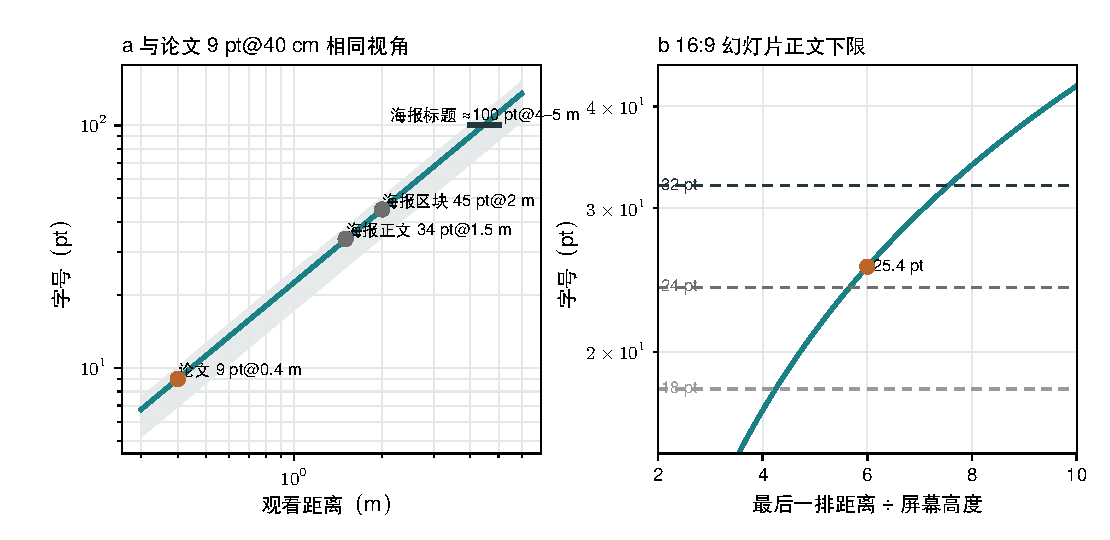
\includegraphics[width=\linewidth]{figures/ch12/ch12-02-visual-angle-text-size-zh.pdf}
\caption{由视角换算的字号。曲线给出与在 40 cm 处阅读 9 pt 文字相同的视角所需字号；这是几何推算，不是期刊或会议规定。投影较暗、观众视力或语言条件不利时应进一步放大。}\label{fig:ch12-02}
\end{figure}

下面我们分论文、海报和口头汇报三个场景，逐步推算图~\ref{fig:ch12-02} 中的曲线与关键工作点。

\textbf{第一，建立论文阅读基准。}在阅读纸质期刊或平板电脑时，常见阅读距离约为 $d_0 = 40\ \text{cm} = 400\ \text{mm}$。期刊正文与清晰图表标注常用的字号约为 $s_0 = 9\ \text{pt}$（标称字高 $h_0 = 9 \times 0.3528 \approx 3.18\ \text{mm}$；期刊配图允许的最小刻度字号通常在 $7\text{--}8\ \text{pt}$ 左右）。以“在 $40\ \text{cm}$ 处阅读 $9\ \text{pt}$ 文字”作为本书的参照基准，其对应的张角为：
\[
\theta_0 \approx \frac{3.18\ \text{mm}}{400\ \text{mm}} \approx 0.00794\ \text{rad} \approx 0.45^\circ
\]
如果把论文配图中常见的 $7\text{--}10\ \text{pt}$ 范围一并换算，在 $40\ \text{cm}$ 处对应的视角范围约为 $0.35^\circ\text{--}0.50^\circ$（即图~\ref{fig:ch12-02}a 中的浅灰色阴影带）。这里要特别说明：“$40\ \text{cm}$ 处的 $9\ \text{pt}$”是我们为了方便心算而选定的几何参照点，并不是哪家期刊或国际标准组织的强制规定。

\textbf{第二，按实际打印尺寸换算海报字号（图~\ref{fig:ch12-02}a）。}学术海报通常按 1:1 的物理尺寸排版并打印。因此，要让站在距离海报 $d$（单位：$\text{m}$）处的观众获得与“$0.4\ \text{m}$ 处读 $9\ \text{pt}$”完全相同的视角，所需的海报字号 $s_{\text{poster}}$ 只需按距离倍数线性放大：
\[
s_{\text{poster}}(d) = 9 \times \frac{d}{0.4\ \text{m}}\ \text{pt} = 22.5\,d\ \text{pt}
\]
将上一节海报展区的三个典型阅读距离代入上式，立刻可以得到三层信息的基准字号：
\begin{itemize}
\item \textbf{细节层与近距阅读（$d = 1.0\text{--}1.5\ \text{m}$）：}当观众停步走近到 $1.0\ \text{m}$ 时，等效字号为 $9 \times 1.0 / 0.4 = 22.5\ \text{pt}$；若观众站在 $1.5\ \text{m}$ 处（常见于两人并排站在展板前阅读或讨论），等效字号为 $9 \times 1.5 / 0.4 = 33.75\ \text{pt} \approx 34\ \text{pt}$（图~\ref{fig:ch12-02}a 中间的深灰圆点）。因此，海报上需要在 $1.5\ \text{m}$ 处轻松看清的正文要点与数据图坐标轴，字号设在 $28\text{--}34\ \text{pt}$ 才有几何保障；即便是供 $0.5\text{--}1.0\ \text{m}$ 近看的方法细则或参考文献，也不宜低于 $24\ \text{pt}$。
\item \textbf{结论层标题（$d = 2.0\ \text{m}$）：}为了让站在两米外或斜侧方的观众一眼捕捉到每个证据区块的结论句，代入 $d = 2.0\ \text{m}$ 可得 $9 \times 2.0 / 0.4 = 45\ \text{pt}$。
\item \textbf{顶部主标题带（$d = 4.0\text{--}5.0\ \text{m}$）：}为了让通道上的路过者在四五米外看清研究问题，代入 $d = 4.5\ \text{m}$ 可得 $9 \times 4.5 / 0.4 \approx 101\ \text{pt}$（对应 $4\text{--}5\ \text{m}$ 区间的 $90\text{--}113\ \text{pt}$，图~\ref{fig:ch12-02}a 右上方的深色横线段）。
\end{itemize}

\textbf{第三，用“距离与屏幕高度之比”换算汇报幻灯片字号（图~\ref{fig:ch12-02}b）。}幻灯片与海报有一点本质不同：你排好一页 16:9 幻灯片后，它最终在会场里有多大，取决于报告厅投影屏幕的物理高度 $H$。在 PowerPoint 或 Keynote 的标准 16:9 宽屏设置中，画布尺寸为 $13.333 \times 7.5\ \text{in}$（即 $33.867 \times 19.05\ \text{cm}$），画布总高度固定对应 $7.5 \times 72 = 540\ \text{pt}$。当你在幻灯片上使用字号 $s_{\text{slide}}$（单位：$\text{pt}$）时，单个字符占整个屏幕高度的比例就是 $s_{\text{slide}} / 540$。设会场屏幕的物理高度为 $H$，最后一排听众到屏幕的距离为 $D$，则字符在最后一排听众眼中的张角为：
\[
\theta \approx \frac{(s_{\text{slide}} / 540)\,H}{D} = \frac{s_{\text{slide}}}{540 \times (D/H)}
\]
反过来，若要求最后一排听众看到的视角达到 $\theta_0 \approx 0.45^\circ \approx 0.00785\ \text{rad}$，则幻灯片字号只需由无量纲比值 $D/H$（最后一排距离除以屏幕高度）决定：
\[
s_{\text{slide}} \approx 0.00785 \times \left(\frac{D}{H}\right) \times 540\ \text{pt} \approx 4.24 \times \left(\frac{D}{H}\right)\ \text{pt}
\]
我们看两个具体算例。算例一：某标准学术报告厅的投影屏幕高 $H = 2.0\ \text{m}$（16:9 屏幕宽约 $3.56\ \text{m}$），最后一排距屏幕 $D = 12\ \text{m}$，此时距离与屏高之比 $D/H = 6$。如果在幻灯片上使用 $24\ \text{pt}$ 文字，字符占屏高的 $24 / 540 = 1 / 22.5$，投影到幕布上高约 $8.9\ \text{cm}$，在 $12\ \text{m}$ 处的张角约为 $0.42^\circ$；若按 $0.45^\circ$ 严格计算，所需字号约为 $25.4\ \text{pt}$（图~\ref{fig:ch12-02}b 中的橙褐色圆点）。这就从几何上解释了一条非常实用的经验法则：\textbf{当会场最后一排距离不超过屏幕高度的 6 倍（$D/H \le 6$）时，24 pt 是幻灯片正文与轴标题较为稳妥的下限，坐标刻度也不宜小于 20 pt。}

算例二：如果换到一间狭长的教室，屏幕高只有 $H = 1.5\ \text{m}$，而后排距离达到 $D = 8\ \text{m}$（$D/H \approx 5.33$），此时若在图中使用 $18\ \text{pt}$ 的小字（占屏高 $1/30$），在 $8\ \text{m}$ 处的张角只有 $(1.5 / 30) / 8 \approx 0.00625\ \text{rad} \approx 0.36^\circ$，已经退化到接近论文最小字号的下限（顺便留意，图~\ref{fig:ch12-02}b 左缘的参考线文字 \texttt{18 pt}、\texttt{24 pt}、\texttt{32 pt} 紧贴左轴框内侧并压在了水平虚线上，自己在制作参考线标注时，最好把文字放在虚线上方或右端空白处以避开线条）。

\textbf{第四，同步换算线宽与数据标记。}视角原理同样适用于曲线粗细、坐标轴边框、刻度线和散点符号。在 $40\ \text{cm}$ 处阅读论文时，$0.5\text{--}0.8\ \text{pt}$ 的坐标轴线与 $1.2\ \text{pt}$ 的数据曲线清晰利落；但如果把 $0.5\ \text{pt}$ 细线原封不动放到 $1.5\ \text{m}$ 外观看的海报上，需按距离放大 $1.5 / 0.4 = 3.75$ 倍才能保持同等视觉粗细。因此，幻灯片与海报上的数据曲线和轴线应加粗到 $2.0\text{--}3.5\ \text{pt}$。此外，遇到投影仪发暗、环境光过强、听众坐在大角度侧排或阅读非母语术语时，都应在几何推算值的基础上进一步放大。

\section{从论文组图拆出一组汇报页}

现在回到小周的钙钛矿太阳能电池案例。我们先把第 9 章定稿的论文版 Figure 2（图~\ref{fig:ch12-03}）摆在面前，看看它为什么适合论文，却不适合直接放进幻灯片。

\begin{figure}[htbp]\centering
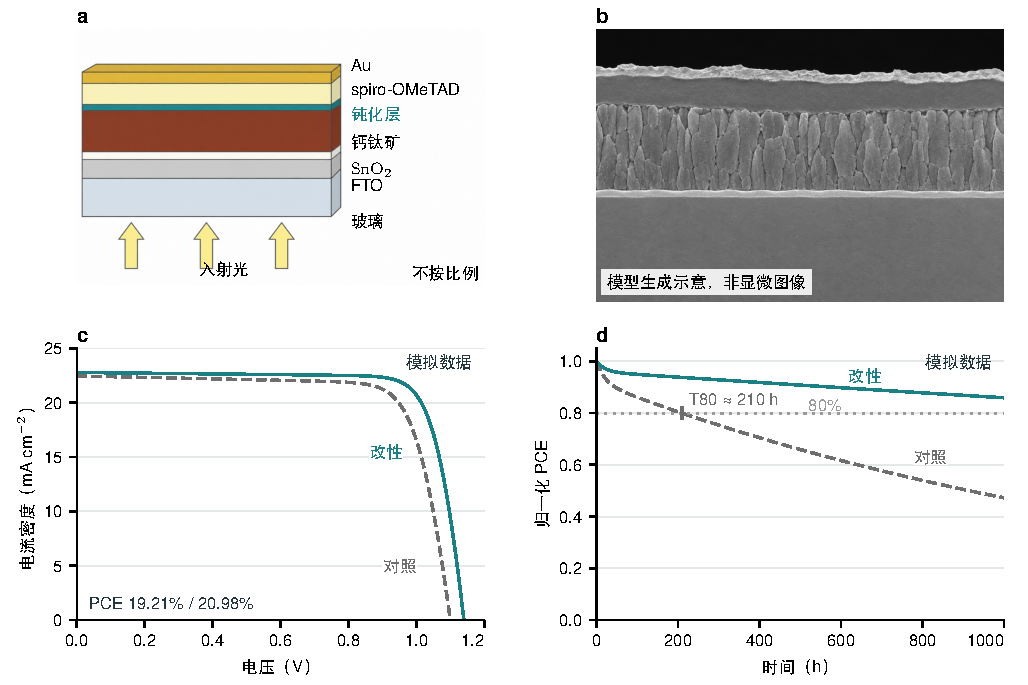
\includegraphics[width=\linewidth]{figures/ch12/ch12-03-paper-figure-2-zh.pdf}
\caption{论文版 Figure 2（第 9 章）。c、d 为模拟数据；b 为模型生成示意，非显微图像；a 不按比例。}\label{fig:ch12-03}
\end{figure}

在图~\ref{fig:ch12-03} 中，四个面板按 $2 \times 2$ 网格紧凑排列在 $174 \times 116\ \text{mm}$ 的双栏画布上：上排左侧面板 a 用七层色块交代玻璃、FTO、$\text{SnO}_2$、钙钛矿、青色钝化层、spiro-OMeTAD 与 Au 背电极的叠层顺序，并在右下角注明“不按比例”；上排右侧面板 b 放置灰度类 SEM 截面图样，左下角用浅白底框明确标注“模型生成示意，非显微图像”；下排面板 c 与 d 分别绘制模拟 $J\text{--}V$ 曲线与 $1000\ \text{h}$ 归一化 PCE 稳定性曲线，统一使用灰色虚线代表对照、青色实线代表改性，并在右上角标明“模拟数据”。然而，当小周把图~\ref{fig:ch12-03} 整张贴进 16:9 幻灯片，并在会场最后一排观看时，效果就变成了图~\ref{fig:ch12-05}a。

\begin{figure}[htbp]\centering
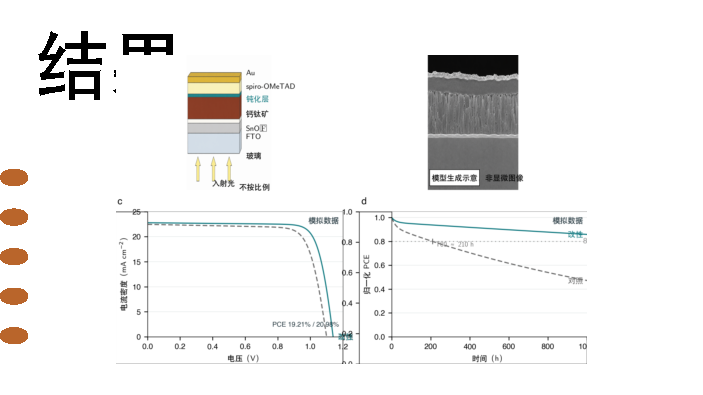
\includegraphics[width=119mm]{figures/ch12/ch12-05a-pasted-zh.pdf}\\[1mm]
{\footnotesize (a) 直接贴入论文组图：左侧橙褐色圆点 (1)--(5) 对应正文分析的五项问题}\\[3mm]
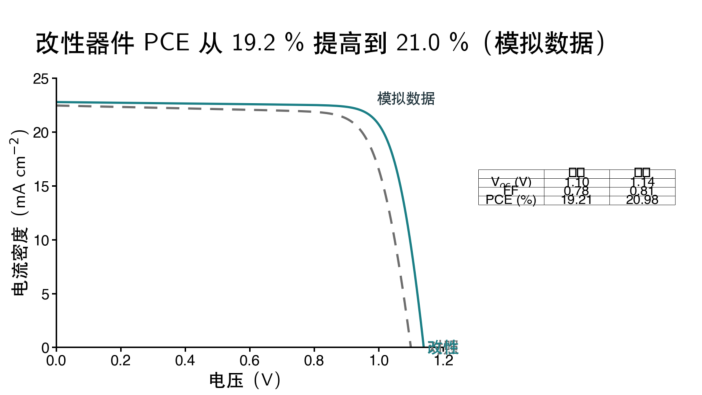
\includegraphics[width=119mm]{figures/ch12/ch12-05b-rebuilt-zh.pdf}\\[1mm]
{\footnotesize (b) 按汇报条件重绘的第 2b 页：单一问题、结论标题与大字号直接标注}
\caption{同一页内容从会场最后一排看到的大小。两图按 119 mm 宽印刷：在 40 cm 处阅读它们，与在 12 m 外看 3.6 m 宽的屏幕视角相同。（a）直接贴入论文组图；（b）按汇报重绘。数据为模拟数据。}\label{fig:ch12-05}\label{fig:ch12-05a}\label{fig:ch12-05b}
\end{figure}

图~\ref{fig:ch12-05} 的印刷宽度经过了精确的视角匹配：在 $12\ \text{m}$ 外看宽 $3.56\ \text{m}$ 的 16:9 投影屏幕，横向视角与在 $40\ \text{cm}$ 处看宽 $119\ \text{mm}$ 的书页完全相同（$3.56 / 12 \times 400\ \text{mm} \approx 119\ \text{mm}$）。因此，两图在书中固定按 $119\ \text{mm}$ 宽印刷，读者在正常阅读距离看到的正是后排听众眼中的真实画面。沿着图~\ref{fig:ch12-05}a 左侧页边的五个橙褐色编号圆点 (1)--(5)，可以清楚看到“整张贴图”暴露出的五项问题：
\begin{enumerate}
\item \textbf{刻度与轴标题过小（对应圆点 1）：}把 $174\ \text{mm}$ 宽、$8\ \text{pt}$ 字（或 $180\ \text{mm}$ 宽、$7\ \text{pt}$ 字）的组图缩放到占 16:9 页面宽度 $90\%$（约 $305\ \text{mm}$）时，在幻灯片坐标系中的等效字号只有约 $12\text{--}14\ \text{pt}$。放到 $12\ \text{m}$ 处观看，视角仅约 $0.21^\circ\text{--}0.25^\circ$，不到论文阅读视角的一半，后排听众根本看不清横轴电压和纵轴电流密度。
\item \textbf{标注挤压、边框重叠与识别困难（对应圆点 2）：}若原论文图使用角落里的独立图例框，听众需要在图例和曲线间来回对照；而即便原图使用了直接标注，在贴图重采样与窄高画布压缩下，图~\ref{fig:ch12-05}a 下排面板 c 的右框线与面板 d 的左轴刻度（\texttt{1.0}、\texttt{0.8}、\texttt{0.6}）直接叠在一起，面板 c 右下角的“对照/改性”与刻度 \texttt{1.2} 撞成一团，面板 d 中的 \texttt{T80} 标注也压在了灰色虚线上。
\item \textbf{四个面板同时争夺注意力（对应圆点 3）：}四个面板同时亮在屏幕上，讲者讲面板 c 时听众却在看面板 a 或 b；且粗暴贴图造成了边缘裁切——上排面板字母 \texttt{a}、\texttt{b} 被裁掉，面板 d 横轴最右侧的 \texttt{1000} 被截成了 \texttt{10}。
\item \textbf{页标题没有结论（对应圆点 4）：}页面左上角只写了“结果”二字（且在图~\ref{fig:ch12-05}a 中因文本框裁切只露出左半边），没有传递任何科学发现。
\item \textbf{证据状态声明受损或丢失（对应圆点 5，诚信高风险项）：}原本写在论文图注里的模拟条件随截图一起丢失；面板 b 左下角的“模型生成示意，非显微图像”在贴图重绘时，“非显微图像”五个黑字溢出了白色底框、落在了深灰色背景上，在后排视角下几乎无法辨认（面板 a 中 $\text{SnO}_2$ 的下标也因字体缺字变成了方框），极易让听众把模型生成的示意形貌误认为真实电镜照片。
\end{enumerate}

要把图~\ref{fig:ch12-03} 改造成像图~\ref{fig:ch12-05}b 那样在后排依然清晰的汇报页，应按以下六个步骤，将空间并列的论文组图重构为时间顺序化的 16:9 幻灯片序列（图~\ref{fig:ch12-04}）：

\begin{figure}[htbp]\centering
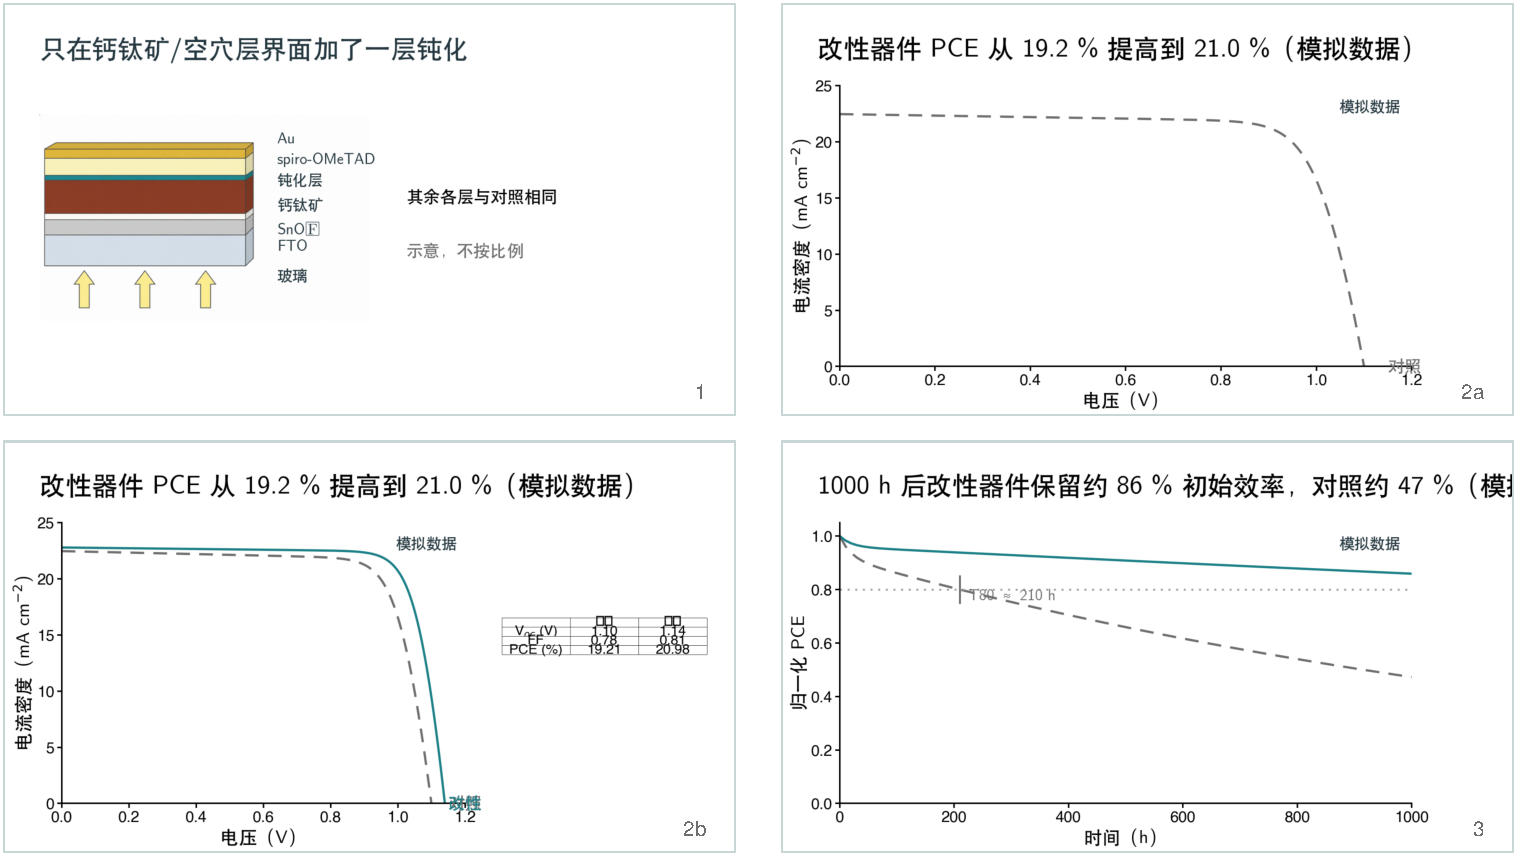
\includegraphics[width=\linewidth]{figures/ch12/ch12-04-slide-sequence-zh.pdf}
\caption{由同一组数据拆出的三页汇报（第 2 页分两步）。每页标题是结论句，图中直接标注曲线；数值、坐标范围与颜色语义与论文版一致。数据为模拟数据。}\label{fig:ch12-04}
\end{figure}

\textbf{第一步，列出组图回答的子问题，把次要面板移入备用页。}论文 Figure 2 依次回答三个核心问题：(1) 器件结构做了什么改动？(2) 初始效率提高了多少？(3) 运行 $1000\ \text{h}$ 后的稳定性改善了多少？面板 b 的类 SEM 截面示意不承担主结论的定量证明，因此不放进 3 分钟的正文汇报页，而是连同完整的“模型生成示意，非显微图像”标注移入报告末尾的备用页，留待问答环节调用。

\textbf{第二步，每页只回答一个子问题，把页标题写成完整结论句。}采用常见的“断言—证据（assertion--evidence）”写法（Naegle，2021），在每页顶部用 $32\text{--}36\ \text{pt}$ 直接写出本页结论并保留证据性质标注：第 1 页写“只在钙钛矿/空穴层界面加了一层钝化”，第 2 页写“改性器件 PCE 从 $19.2\%$ 提高到 $21.0\%$（模拟数据）”，第 3 页写“$1000\ \text{h}$ 后改性器件保留约 $86\%$ 初始效率，对照约 $47\%$（模拟数据）”。

\textbf{第三步，设计分步揭示（progressive reveal）。}将第 2 页拆为完全对齐的两帧（第 2a 页与第 2b 页）：先切出第 2a 页，画面上只有坐标轴与灰色虚线“对照”曲线，讲者口头带听众读懂横纵坐标含义；随后翻到第 2b 页（即图~\ref{fig:ch12-05}b），在横纵坐标范围分毫不差的同一坐标系上，叠加青色实线“改性”曲线并在右侧亮出 $V_{\text{oc}}$、$\text{FF}$ 与 $\text{PCE}$ 简表。两帧坐标范围完全一致，翻页时曲线不跳动，听众能立即看清改性带来的增量。

\textbf{第四步，删去面板字母与长图例，改为直接标注。}删去 \texttt{a}--\texttt{d} 面板字母和独立图例框，在曲线旁直接标“对照”“改性”，并在第 1 页器件结构图上用橙褐色粗框高亮新增的钝化层，右侧只留两行要点（“其余各层与对照相同”“示意，不按比例”）。

\textbf{第五步，按 16:9 原生尺寸重绘，并放大检查排版细节。}每页按 $13.333 \times 7.5\ \text{in}$ 原生画布绘制（页标题 $34\ \text{pt}$，轴标题 $24\ \text{pt}$，刻度 $20\ \text{pt}$，标注 $22\ \text{pt}$，线宽 $3\ \text{pt}$），绝不拉伸原图。同时，对照图~\ref{fig:ch12-04} 的实际出图画面做原尺寸复查，能抓出四处需要在上台前修正的细节：(1) 第 1 页层名中的 $\text{SnO}_2$ 若直接使用 Unicode 下标字符，在中文字体下会因缺字变成方框，应改为数学模式 \texttt{\$\textbackslash mathrm\{SnO\_2\}\$} 或在演示软件中用文本框下标；(2) 第 2a、2b 页若把直接标注简单绑在曲线最末一个点（$J = 0$）右侧，“对照”与“改性”会叠在横轴右端并与刻度 \texttt{1.2} 碰撞（图~\ref{fig:ch12-05}b 右下角同样可见），应将标签上移到曲线陡降段的中部空白处；(3) 第 2b 页右侧用绘图函数生成小表时，表头单元格因未显式绑定中文字体出现了两个方框且行高偏紧，实际制作幻灯片时直接在 PowerPoint 中插入原生表格更稳妥；(4) 第 3 页标题字数较多，单行 $34\ \text{pt}$ 在画布右缘被截掉半个括号，应手动换行或微调至 $30\ \text{pt}$。

\textbf{第六步，保持数值、坐标范围、颜色语义与证据声明一致。}全部数值、轴范围（$0\text{--}1.2\ \text{V}$，$0\text{--}25\ \text{mA cm}^{-2}$，$0\text{--}1000\ \text{h}$；若改变范围须在讲稿中说明）、灰虚线对照与青实线改性、以及图内右上角的“模拟数据”标注，均与论文版保持严格一致。

\section{A0 竖版海报：栅格、层次与密度}

按照国际标准 ISO 216，\textbf{A0 竖版海报}的物理尺寸为 $841 \times 1189\ \text{mm}$，面积恰好为 $1\ \text{m}^2$。规划海报版面之前，先看展厅里的真实观看过程（图~\ref{fig:ch12-07}）。

\begin{figure}[htbp]\centering
\begin{tikzpicture}
\node[anchor=south west,inner sep=0] (img) at (0,0) {
\includegraphics[width=\linewidth]{figures/ch12/ch12-07-poster-hall-distances.png}};
\begin{scope}[x={(img.south east)},y={(img.north west)}]
  \node[font=\footnotesize,fill=white,fill opacity=0.88,text opacity=1,inner sep=2pt] at (0.18,0.12) {约 3--5 m：读标题与主结论};
  \node[font=\footnotesize,fill=white,fill opacity=0.88,text opacity=1,inner sep=2pt] at (0.58,0.12) {约 1 m：读证据与细节};
\end{scope}
\end{tikzpicture}
\caption{海报先被远看，再被近看。示意图，人物与距离不按比例（底图由图像模型生成，距离标签由作者后期叠加；提示词与生成记录见本书仓库）。}\label{fig:ch12-07}
\end{figure}

生成图~\ref{fig:ch12-07} 的无字底图时，同一段英文提示词连续调用了三次：第 1 次生成中地面两条浅灰虚线的倾斜方向分歧明显，第 2 次远距虚线绕到了行走者身后，第 3 次才使两条虚线分别经过左前景行走者脚边与中间驻足阅读者前方，且五块展板只包含蓝青标题色带、两栏浅灰矩形与无字几何图形（底图保留了柔和渐变且展板排占了右侧约四分之三，距离标签由 TikZ 在排版时叠加）。图中直观展示了海报的“两阶段阅读”：通道上约 $3\text{--}5\ \text{m}$ 外的路过者用几秒钟扫视顶部标题带；被吸引而走到约 $1\ \text{m}$ 处的同行则用几分钟依次阅读证据区块与方法细节。

顺应这一过程，我们为 A0 竖版海报设计\textbf{两栏栅格}与\textbf{三层信息结构}（图~\ref{fig:ch12-06}）。

\begin{figure}[htbp]\centering
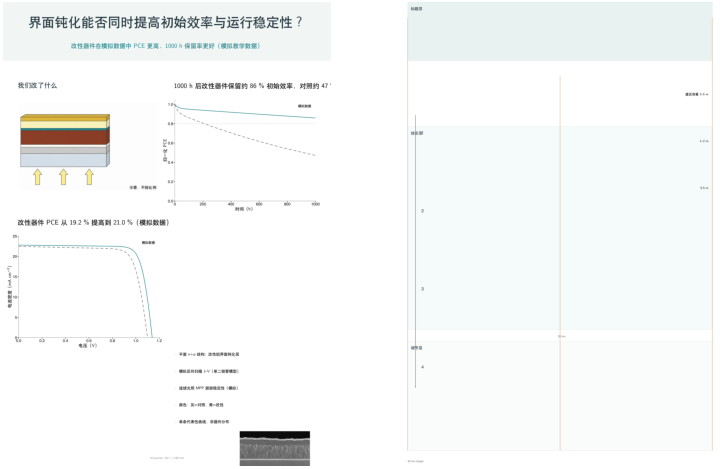
\includegraphics[width=\linewidth]{figures/ch12/ch12-06-a0-poster-layout-zh.pdf}
\caption{A0 竖版海报（$841 \times 1189\ \text{mm}$）的终稿与线框。三层信息分别面向 $3\text{--}5\ \text{m}$、$1\text{--}2\ \text{m}$ 与 $0.5\ \text{m}$ 的阅读；数据图按 $1.5\ \text{m}$ 观看重绘。数据为模拟数据；截面图为模型生成示意。}\label{fig:ch12-06}
\end{figure}

对照图~\ref{fig:ch12-06} 的终稿与线框，A0 竖版海报的布局要点如下：
\begin{enumerate}
\item \textbf{栅格与按栏向下的阅读顺序：}四周留出 $30\ \text{mm}$ 外边距（建议 $\ge 25\ \text{mm}$），顶部设高 $150\ \text{mm}$ 的通栏标题带，主体分为左右两栏，栏间距 $20\ \text{mm}$（建议 $15\text{--}20\ \text{mm}$），单栏净宽 $380.5\ \text{mm}$。阅读顺序按栏从上到下推进（先读左栏上、左栏下，再读右栏上、右栏下，如线框图左侧箭头与编号 \texttt{1}--\texttt{4} 所示），避免观众在近一米宽的展板前左右来回走动（Erren 与 Bourne，2007）。
\item \textbf{三层信息与论文四个面板的重新分工：}
  \begin{itemize}
  \item \textbf{标题层（面向 $3\text{--}5\ \text{m}$）：}顶部浅青灰底色带内，第一行用 $96\ \text{pt}$ 写出研究问题“界面钝化能否同时提高初始效率与运行稳定性？”，第二行用 $44\ \text{pt}$ 青色副标题写出主结论“改性器件在模拟数据中 PCE 更高、$1000\ \text{h}$ 保留率更好（模拟教学数据）”。
  \item \textbf{结论层（面向 $1\text{--}2\ \text{m}$）：}中上部三个核心区块分别对应左栏上“我们改了什么”（器件结构 M1，配 $28\ \text{pt}$“示意，不按比例”）、左栏下效率区块（$J\text{--}V$）和右栏上稳定性区块。每个数据区块顶部配 $48\ \text{pt}$ 结论句，下方数据图按 $1.5\ \text{m}$ 距离专门重绘（轴标题 $32\ \text{pt}$、刻度 $28\ \text{pt}$、线宽 $3.5\ \text{pt}$、右上角“模拟数据” $24\ \text{pt}$）。
  \item \textbf{细节层（面向 $0.5\ \text{m}$）：}右栏下区块用 5 条 $28\ \text{pt}$ 短要点交代平面结构、单二极管模拟、MPP 条件、灰/青颜色定义与单条代表性曲线说明；论文 Figure 2 的面板 b（类 SEM 截面示意 M2）降级移至右下角细节层，并保留 $24\ \text{pt}$ 证据声明。
  \end{itemize}
  按 100\% 尺寸核查图~\ref{fig:ch12-06} 左图的脚本排样时，也能发现送印前需要人工修补的三处细节：一是右栏上稳定性区块的 $48\ \text{pt}$ 结论句较长，单行排布时右端括号在栏边被裁掉一半，应拆成两行或缩至 $44\ \text{pt}$；二是左栏上器件结构图 M1 仅放了无字底图，送印前需补上右侧 $36\ \text{pt}$ 的七层层名标签及数据图内的曲线旁注；三是右下角截面图 M2 左下方的深色标注“模型生成示意，非显微图像”直接叠在深灰基底上对比度不足，应加上浅白半透明底框。
\item \textbf{密度指标与眯眼测试（squint test）：}海报正文总字数建议用“能否在 5 分钟内读完”自测，并保持充足留白。排版后将海报缩至 $12\ \text{cm}$ 高并施加高斯模糊（$\sigma$ 约相当于缩略图上 $1.5\ \text{mm}$），开展\textbf{眯眼测试}（图~\ref{fig:ch12-08}）。
\end{enumerate}

\begin{figure}[htbp]\centering
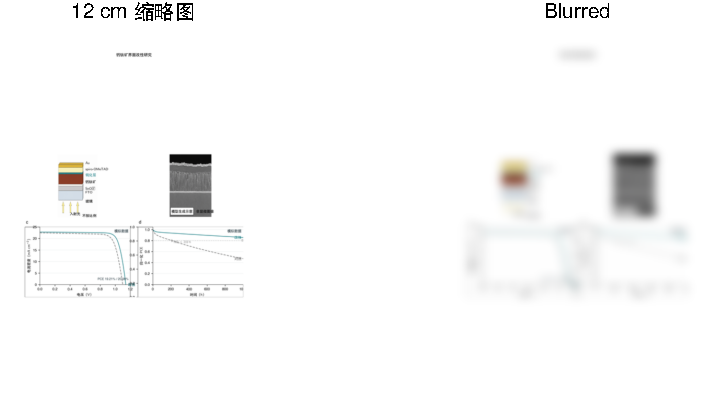
\includegraphics[width=\linewidth]{figures/ch12/ch12-08a-dense-squint-zh.pdf}\\[1mm]
{\footnotesize (a) 拥挤初稿 C0：三栏文字加原样放大的四面板论文组图}\\[3mm]
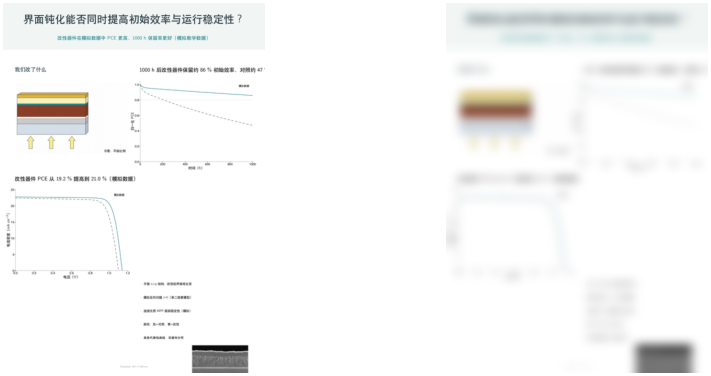
\includegraphics[width=\linewidth]{figures/ch12/ch12-08b-focused-squint-zh.pdf}\\[1mm]
{\footnotesize (b) 分层终稿：顶部标题带、三个结论区块与右下细节层}
\caption{眯眼测试。左：12 cm 高的缩略图；右：模糊后。（a）拥挤初稿只剩均匀灰块；（b）终稿仍能看出标题带和三个区块。}\label{fig:ch12-08}\label{fig:ch12-08a}\label{fig:ch12-08b}
\end{figure}

对比图~\ref{fig:ch12-08}a 与图~\ref{fig:ch12-08}b（注：图~\ref{fig:ch12-08}a 左上方的子图标题因未显式传入中文字体属性出现了三个方框）：拥挤初稿 C0 在顶部只放了 $36\ \text{pt}$ 的小标题“钙钛矿界面改性研究”，上半幅分三栏铺排摘要、引言、方法、结果与讨论、结论五段 $20\ \text{pt}$ 正文（样张共约 230 字），中部把 $174\ \text{mm}$ 宽的论文 Figure 2 等比放大约 $4$ 倍横跨版面（$0.6\ \text{pt}$ 线变成约 $2.4\ \text{pt}$ 尚可，但 $8\ \text{pt}$ 字只变成约 $32\ \text{pt}$，与正文同级而使层次消失）。模糊后，顶部标题与三栏文字化作浅灰影，看不出主结论与区块分工；而终稿（图~\ref{fig:ch12-08}b）模糊后仍能清晰分辨顶部浅青标题带、三个带粗结论横条的区块以及右下细节层。

\section{在 SciDraw AI 中完成三个版本}

在 \scidraw{} 中完成论文、汇报与海报三个版本时，应按具体任务选用对应入口，并分清哪些步骤由平台完成、哪些步骤须由作者在本地软件中复核：
\begin{itemize}
\item \textbf{数据图改画幅与字号重绘（科学可视化 \sdtool{sci-vis}）：}无需重新上传数据表，直接打开第 9 章论文图的历史会话，选中终稿版本继续输入修改指令，即可生成 16:9 汇报版、仅含对照曲线的分步揭示版以及海报图块版。平台支持多轮对话修改、历史版本继续编辑、恢复上一版或原版以及多格式导出。作者需逐项核对数值、坐标范围与颜色语义是否未变，并在 PowerPoint 或海报页面中按实际物理尺寸复核字号（导出格式是否为可编辑真矢量将在第 13 章详述）。
\item \textbf{汇报页框架与海报排版框架（演示模板 \path{/scientific-presentation-templates} 与海报模板）：}演示模板提供学位答辩、会议报告、文献汇报、组会汇报、开题报告等场景的 16:9 PPTX 框架；海报模板提供“经典”“焦点”“四栏”三种风格，尺寸覆盖 A0 竖版、A0 横版、A1、$36\times 48\ \text{in}$、$90\times 120\ \text{cm}$ 与 16:9 电子海报等变体（其中 $72\ \text{in}$ 超宽海报受限于演示软件单页尺寸上限，按 $50\%$ 物理尺寸设计、打印时放大 2 倍，模板内有明确注明）。注意：\textbf{下载 PPTX 模板不等于自动填入内容}，平台目前没有“一键把整篇论文自动排成多页可编辑演示或可编辑海报”的功能，作者需自己将重绘好的图片与结论句排入模板。
\item \textbf{海报整体视觉方向探索（科学海报生成 \path{/scientific-poster-maker}）：}可根据提示词生成单张海报概念图像，也支持导入论文 PDF 生成视觉提示词（目前 PDF 解析仅读取前 5 页及摘要、开头有限文本，并非理解整篇论文）。该工具仅用于开工前比较分栏与配色方向；\textbf{严禁把生成的单张位图直接当成终稿送印}，生成图中的任何文字与假“数据图”一律不用，最终版必须在可编辑模板或脚本中用真实内容排版。
\item \textbf{组图拆解与目标宽度技术检查（组图工具 \sdtool{multi-panel-figure-maker} 与图片检查器 \sdtool{figure-checker}）：}组图工具导出的 PPTX 中，每个面板位图与面板编号文字（\texttt{a}、\texttt{b}……）彼此独立，便于单独提取面板 a 的结构图或删去编号；但面板内部的曲线、坐标轴与文字仍是位图，不可逐根编辑，因此数据面板仍须回 \sdtool{sci-vis} 或脚本按汇报字号重绘。定稿后可用 \sdtool{figure-checker} 按目标物理宽度换算有效分辨率并检查灰度与色觉风险，但字号张角、版面阅读顺序与科学表述仍须由作者用视角公式与眯眼测试自己核查。各工具之间通过下载命名清楚的文件再上传或插入完成交接。
\end{itemize}

\section{完整案例：一项研究的三个版本}

下面将本章钙钛矿太阳能电池界面改性研究从原始材料、三份任务书、修改指令到讲稿、图注与三版一致性核验完整串联起来。

\textbf{一、研究设定与模拟数据参数。}本案例比较平面 n-i-p 钙钛矿太阳能电池的对照器件与界面钝化改性器件，不报告任何真实器件实验结果，所有数据均由标准单二极管模型与给定双指数衰减函数生成。器件自下而上依次为：玻璃 / FTO / $\text{SnO}_2$（约 $30\ \text{nm}$）/ 钙钛矿吸光层（约 $500\ \text{nm}$）/ 界面钝化层（仅改性组，极薄）/ spiro-OMeTAD（约 $200\ \text{nm}$）/ Au（约 $80\ \text{nm}$），不指定具体钙钛矿组分或钝化分子。

四份材料中，M1 为器件结构示意图（不按比例）；M2 为模型生成的类 SEM 截面示意（真实论文中截面形貌必须来自同批器件的实际 SEM 采集并保留原图与比例尺，本书仅因无法公开获取与模拟数据同源的真实照片而用模型图样作版式占位，所有衍生版本均须标明“模型生成示意，非显微图像”）；M3 为 AM1.5G（$100\ \text{mW cm}^{-2}$）、$25\ ^\circ\text{C}$ 下的单二极管模拟 $J\text{--}V$ 曲线（单一反向扫描，未模拟迟滞，迟滞问题参见 Snaith 等，2014；效率理论上限参见 Shockley 与 Queisser，1961），对照组设定 $J_L = 22.5\ \text{mA cm}^{-2}$、目标 $V_{\text{oc}} = 1.10\ \text{V}$、$n = 1.6$、$R_s = 2.5\ \Omega\cdot\text{cm}^2$、$R_{\text{sh}} = 1500\ \Omega\cdot\text{cm}^2$，计算输出 $J_{\text{sc}} = 22.46\ \text{mA cm}^{-2}$、$V_{\text{oc}} = 1.100\ \text{V}$、$\text{FF} = 0.777$、$\text{PCE} = 19.21\%$，改性组设定 $J_L = 22.8\ \text{mA cm}^{-2}$、目标 $V_{\text{oc}} = 1.14\ \text{V}$、$n = 1.5$、$R_s = 2.0\ \Omega\cdot\text{cm}^2$、$R_{\text{sh}} = 3000\ \Omega\cdot\text{cm}^2$，计算输出 $J_{\text{sc}} = 22.78\ \text{mA cm}^{-2}$、$V_{\text{oc}} = 1.140\ \text{V}$、$\text{FF} = 0.808$、$\text{PCE} = 20.98\%$；M4 为连续 1 个太阳光照、最大功率点跟踪、氮气、约 $25\ ^\circ\text{C}$ 下的 $0\text{--}1000\ \text{h}$ 归一化 PCE 模拟序列（稳定性评估与报告共识参见 Khenkin 等，2020），对照组 $y(t) = [1 - 0.08(1 - e^{-t/20})]e^{-t/1500}$ 的 $T_{80} = 210\ \text{h}$、$1000\ \text{h}$ 保留率 $0.47$，改性组 $y(t) = [1 - 0.04(1 - e^{-t/20})]e^{-t/9000}$ 在 $1000\ \text{h}$ 内未降至 $0.80$（$T_{80} > 1000\ \text{h}$）、$1000\ \text{h}$ 保留率 $0.86$。

\textbf{二、三份任务书。}三个版本各自遵循如下任务书。

任务书 A（论文版 Figure 2）：
\begin{Prompt}
【用途与读者】论文 Figure 2，读者为光伏/材料方向同行，单独阅读，节奏由读者控制。
【一句话目标】读者能看出改性器件在初始效率和 1000 h 稳定性上都优于对照，并能找到 Jsc、Voc、FF、PCE 和 T80。
【面板】a 器件结构；b 截面图样（模型生成示意）；c J–V；d 归一化 PCE–时间。
【尺寸】双栏 174 mm 宽，面板内字号 8 pt，面板字母 10 pt 粗体小写。
【不可改变】全部数值来自统一计算结果文件；颜色语义：对照灰 #6E6E6E 虚线，改性青 #1B7F86 实线。
【标注】c、d 为模拟数据；b 为模型生成示意，非显微图像；a 不按比例。
\end{Prompt}

任务书 B（组会 / 会议汇报版，3 页 16:9）：
\begin{Prompt}
【用途与读者】10 分钟组会报告中的结果部分，约 3 分钟；听众为课题组成员与相近方向同行；
投影屏幕高约 2 m，最后一排约 10–12 m；节奏由讲者控制。
【一句话目标】听众在 3 页内依次理解：器件做了什么改动 -> 初始效率提高了多少 -> 稳定性改善了多少。
【每页】
  第 1 页 标题句：“只在钙钛矿/空穴层界面加了一层钝化”。器件结构（M1）放大，钝化层高亮；
          类 SEM 示意不放入正文页（放备用页，标注保留）。
  第 2 页 标题句：“改性器件 PCE 从 19.2 % 提高到 21.0 %（模拟数据）”。J–V 分两步揭示：
          先坐标轴+对照，再加改性；关键参数用直接标注与简表，不用独立图例。
  第 3 页 标题句：“1000 h 后改性器件保留约 86 % 初始效率，对照约 47 %（模拟数据）”。
          稳定性曲线，标出 0.8 参考线与对照 T80。
【版式】16:9，33.867 x 19.05 cm；正文与刻度 >= 20 pt，轴标题 >= 24 pt，页标题 32–36 pt；线宽 >= 2.5 pt；无面板字母。
【不可改变】数值、轴物理量与单位、颜色语义、“模拟数据”标注。
【验收】在笔记本屏幕上把页面缩到 1/4 大小，标题句与轴标签仍可读；每页数值与结果文件一致。
\end{Prompt}

任务书 C（A0 竖版海报）：
\begin{Prompt}
【用途与读者】学术会议海报展区，A0 竖版 841 x 1189 mm；路过者在 2–5 m 外决定是否停留，
停留者在 0.5–1.5 m 阅读 3–5 分钟；作者不一定在场。
【一句话目标】从 3 m 外读到研究问题与主结论；走近后依次读到“做了什么—效率—稳定性”三块证据和必要方法。
【层次】标题层：研究问题+主结论（标题 >= 90 pt）；结论层：3 个区块，每块一句结论（>= 44 pt）+ 一张图；
细节层：方法要点、参数、参考文献、二维码（正文 >= 28 pt，最小 24 pt）。
【栅格】2 栏，外边距 30 mm，栏间距 20 mm；阅读顺序：标题 -> 左栏上（结构）-> 左栏下（J–V）
-> 右栏上（稳定性）-> 右栏下（方法、截面示意、参考）。
【图】数据图按 1.5 m 观看重绘（刻度 >= 28 pt，线宽 >= 3 pt），不是论文图放大；类 SEM 示意放细节层。
【不可改变】同任务书 B。
【验收】缩到 12 cm 高的缩略图上能分辨 3 个区块和主结论；1:1 打印 A4 局部样张在 1.5 m 处可读。
\end{Prompt}

\textbf{三、可复制的修改指令与海报版式提示词。}对 \sdtool{sci-vis} 中第 9 章的 $J\text{--}V$ 会话（选择论文终稿那一版继续修改），输入如下指令：
\begin{Prompt}
在保持全部数据点、两组颜色（对照 #6E6E6E、改性 #1B7F86）、横轴 0–1.2 V、纵轴 0–25 mA/cm2 不变的前提下，
生成一个用于 16:9 幻灯片的版本：
1. 画布 16:9，图占画面左侧约 60%；
2. 坐标刻度字号相当于 20 pt、轴标题 24 pt（按 33.867 cm 宽的幻灯片计算）；线宽 3 pt；
3. 删除图例，在曲线空白处直接标注“对照”“改性”；
4. 在图内右上角写“模拟数据”；
5. 不添加任何新的数值、误差线或显著性标记。
另外输出一个只有对照曲线的版本（坐标轴、标注相同），用于分步揭示。
\end{Prompt}

生成后需核对两版坐标范围是否完全一致（叠放切换时曲线不能跳动）、标注数值是否与结果文件一致，以及工具是否擅自改动了颜色或平滑了曲线。制作海报版数据图时，只需把上述指令改为“按 A0 海报中宽 $380\ \text{mm}$ 的图块、$1.5\ \text{m}$ 观看距离：刻度 $28\ \text{pt}$、轴标题 $32\ \text{pt}$、线宽 $3.5\ \text{pt}$”。

若使用 \texttt{/scientific-poster-maker} 生成海报版式与视觉方向参考，可输入如下英文提示词：
\begin{Prompt}
A0 portrait academic poster layout for a materials science study, two columns,
clear title band across the top, three large figure blocks with generous white space,
a narrow footer band. Clean flat design, white background, one accent color teal.
Use simple placeholder rectangles for figures and grey bars for text;
do not render any readable words.
\end{Prompt}

\textbf{四、讲稿要点与海报区块图注。}汇报第 2 页（图~\ref{fig:ch12-04} 的 2a $\rightarrow$ 2b，约 40 秒）配套讲稿：
\begin{BookNote}
“先看坐标：横轴是电压，纵轴是电流密度，曲线和两轴围成的矩形越‘方’，填充因子越高。灰线是对照——（点击）青线是改性器件。开路电压从 $1.10\ \text{V}$ 提高到 $1.14\ \text{V}$，填充因子从 $0.78$ 提高到 $0.81$，效率从 $19.2\%$ 到 $21.0\%$。这些是模拟数据，用来说明表达方法。”
\end{BookNote}

海报左栏下 $J\text{--}V$ 区块配套图注：
\begin{BookNote}
改性器件的开路电压与填充因子较高。模拟反向扫描 $J\text{--}V$ 曲线（单二极管模型），AM1.5G，$100\ \text{mW cm}^{-2}$；每组一条代表性曲线，不代表器件间分布。
\end{BookNote}

\textbf{五、三版一致性核验。}最终交付前，对照表~\ref{tab:ch12-02} 逐项核验三个版本的一致性。

\begin{table}[htbp]\centering\footnotesize
\setlength{\tabcolsep}{3pt}
\renewcommand{\arraystretch}{1.15}
\caption{论文版、汇报版与海报版的三版一致性核验表。}\label{tab:ch12-02}
\begin{tabularx}{\linewidth}{@{}>{\raggedright\arraybackslash}p{26mm}YYY>{\raggedright\arraybackslash}p{16mm}@{}}
\toprule
\textbf{检查项} & \textbf{论文版} & \textbf{汇报版} & \textbf{海报版} & \textbf{是否一致} \\
\midrule
$J_{\text{sc}}$ / $V_{\text{oc}}$ / $\text{FF}$ / $\text{PCE}$（两组） & 结果表与面板 c 标注 & 第 2 页标题与右侧小表 & 左栏下 $J\text{--}V$ 区块 & 逐项一致 \\
$T_{80}$（对照 $\approx 210\ \text{h}$）、$1000\ \text{h}$ 保留率（$0.47$ / $0.86$） & 结果表与面板 d 标注 & 第 3 页标题与图内标注 & 右栏上稳定性区块 & 逐项一致 \\
轴物理量、单位、范围 & $0\text{--}1.2\ \text{V}$；$0\text{--}25\ \text{mA cm}^{-2}$；$0\text{--}1000\ \text{h}$ & 同论文版（2a/2b 完全锁定） & 同论文版 & 是（改变须说明） \\
颜色与线型语义 & 灰虚线=对照，青实线=改性 & 同论文版 & 同论文版 & 是 \\
“模拟数据”标注 & 图注及面板 c、d 右上角 & 每张数据页标题与图内 & 标题带、每张数据图内及细节层 & 是 \\
“模型生成示意，非显微图像” & 图注及面板 b 左下角 & 备用页图内 & 右栏下细节层图内 & 是 \\
新增内容 & — & 无新数值或伪造统计 & 无新数值或伪造统计 & 是 \\
\bottomrule
\end{tabularx}
\end{table}

\section{AI 在这一步能做什么与不能做什么}

把论文配图改造成口头汇报和学术海报时，AI 与作者的职责边界汇总于表~\ref{tab:ch12-01}。

\begin{table}[htbp]\centering\footnotesize
\setlength{\tabcolsep}{3pt}
\renewcommand{\arraystretch}{1.15}
\caption{在汇报与海报制作环节中 AI 能做什么、不能做什么与作者必须核对的内容。}\label{tab:ch12-01}
\begin{tabularx}{\linewidth}{@{}>{\raggedright\arraybackslash}p{18mm}YYY@{}}
\toprule
\textbf{环节} & \textbf{AI 能做} & \textbf{AI 不能做} & \textbf{作者要核对} \\
\midrule
拆分故事 & 根据作者给出的结论句草拟页面顺序、页标题候选 & 判断哪个结果是研究的主要贡献；替你决定删掉哪些证据 & 每页标题句有数据支撑、限定条件没丢（“模拟”“单条曲线”） \\
数据图重绘 & 在 \sdtool{sci-vis} 中按新画幅、字号、线宽重绘；生成分步揭示用的子集版本 & 保证字号在最终投影/打印尺寸下精确；保证没有顺手改动坐标或平滑曲线 & 数值、轴范围、颜色语义与论文版逐项一致；字号在 PowerPoint 实际尺寸复核 \\
海报版式 & 用 \path{/scientific-poster-maker} 生成版式与视觉方向参考；提供 PPTX 海报模板 & 生成可直接印刷、文字正确、数据真实的海报；把论文自动排进模板 & 生成图中的文字与“数据”一律不用；最终版在可编辑模板中排 \\
演示文件 & 提供多种 PPTX 演示模板；组图可导出面板分离的 PPTX & 把论文内容自动排成多页可编辑演示；让面板内曲线可逐条编辑 & 模板只是框架；面板内部是位图 \\
讲稿与图注 & 草拟讲稿与海报短图注 & 编造样本量、统计或未给出的条件 & 讲稿中的每个数字回到结果表；证据状态标注在每个版本都保留 \\
检查 & \sdtool{figure-checker} 按目标宽度换算有效分辨率、色觉风险等 & 判断字号、版面层次、阅读顺序或科学正确性 & 用第 12.2 节的换算和眯眼测试自己查 \\
\bottomrule
\end{tabularx}
\end{table}

\section{本章检查清单}

\begin{itemize}
\item 三个版本各有一份任务书，写明观看距离、时间与节奏控制者。
\item 用视角换算确定了每个版本的最小字号与线宽，并在实际尺寸（PowerPoint 页面 / A0 PDF）中复核。
\item 汇报每页只有一个结论句和一组证据；逐步揭示的各帧坐标范围相同。
\item 汇报和海报中的数据图是重绘的，不是论文图放大或截图。
\item 去掉了面板字母和需要来回对照的图例，改为直接标注。
\item 海报有标题层、结论层、细节层；缩略加模糊后仍能看出主要区块。
\item 三版一致性表逐项核对通过：数值、单位、轴范围、颜色语义一致。
\item “模拟数据”“模型生成示意，非显微图像”“示意，不按比例”等证据标注出现在每一个衍生版本的画面上，而不只在论文图注里。
\item 没有使用海报生成图中的文字或数据；没有把模板下载说成自动排版。
\item 各步输入与重绘文件已按版本妥善归档保存。
\end{itemize}

\section{练习}

\begin{enumerate}
\item \textbf{（算一算：纸笔）}你的报告厅屏幕高 $1.6\ \text{m}$，最后一排距屏幕 $14\ \text{m}$。（a）与 $9\ \text{pt}@40\ \text{cm}$ 相同张角时，16:9 幻灯片正文最小约多少 $\text{pt}$？（b）若会议海报正文要在 $1.8\ \text{m}$ 处读到，至少多少 $\text{pt}$？\\
{\footnotesize \textbf{参考答案：}（a）$D/H = 8.75$，$\text{pt} \approx 0.00785 \times 8.75 \times 540 \approx 37\ \text{pt}$（说明这个会场需要比“$24\ \text{pt}$ 下限”更大的字，或减少每页文字）；（b）$9 \times 1.8 / 0.4 = 40.5\ \text{pt}$。}

\item \textbf{（拆一张自己的组图：\scidraw{} 实操）}选你论文中的一张多面板图，写出它回答的 2--3 个子问题，各写一句结论作为页标题。在 \sdtool{sci-vis} 打开对应数据图的历史会话（或重新上传数据），用第 12.6 节的修改指令格式生成 16:9 版本和分步揭示版本；把两版坐标范围、数值和颜色做成一致性表。提交：页面 PNG、修改指令原文、一致性表。

\item \textbf{（眯眼测试）}下载本章图~\ref{fig:ch12-06} 的海报 PDF 和你自己（或同学）的一张海报，缩到 $12\ \text{cm}$ 高并模糊（或站在 $3\ \text{m}$ 外拍照）。写出：能否看出研究问题、主结论和 3 个区块；若不能，列出三条可执行的修改指令（例如“把‘结果’改为结论句‘……’”，而不是“让海报更清楚”）。
\end{enumerate}

\section*{参考文献}

\begin{itemize}
\item Bourne, P. E. (2007). Ten simple rules for making good oral presentations. \textit{PLoS Computational Biology}, 3(4), e77. \url{https://doi.org/10.1371/journal.pcbi.0030077}
\item Erren, T. C., \& Bourne, P. E. (2007). Ten simple rules for a good poster presentation. \textit{PLoS Computational Biology}, 3(5), e102. \url{https://doi.org/10.1371/journal.pcbi.0030102}
\item Khenkin, M. V., Katz, E. A., Abate, A., Bardizza, G., Berry, J. J., Brabec, C., \ldots{} Lira-Cantu, M. (2020). Consensus statement for stability assessment and reporting for perovskite photovoltaics based on ISOS procedures. \textit{Nature Energy}, 5, 35--49. \url{https://doi.org/10.1038/s41560-019-0529-5}
\item Naegle, K. M. (2021). Ten simple rules for effective presentation slides. \textit{PLOS Computational Biology}, 17(12), e1009554. \url{https://doi.org/10.1371/journal.pcbi.1009554}
\item Rougier, N. P., Droettboom, M., \& Bourne, P. E. (2014). Ten simple rules for better figures. \textit{PLoS Computational Biology}, 10(9), e1003833. \url{https://doi.org/10.1371/journal.pcbi.1003833}
\item Shockley, W., \& Queisser, H. J. (1961). Detailed balance limit of efficiency of p-n junction solar cells. \textit{Journal of Applied Physics}, 32(3), 510--519. \url{https://doi.org/10.1063/1.1736034}
\item Snaith, H. J., Abate, A., Ball, J. M., Eperon, G. E., Leijtens, T., Noel, N. K., \ldots{} Wiesner, U. (2014). Anomalous hysteresis in perovskite solar cells. \textit{The Journal of Physical Chemistry Letters}, 5(9), 1511--1515. \url{https://doi.org/10.1021/jz500113x}
\end{itemize}
